\chapter{Control System}
This section describes the control system used for both the fixed and variable pitch quadrotors. It explains how basic PID controllers work and how they are utilized in this project. \bigskip
\begin{figure}[H]
          \centering
            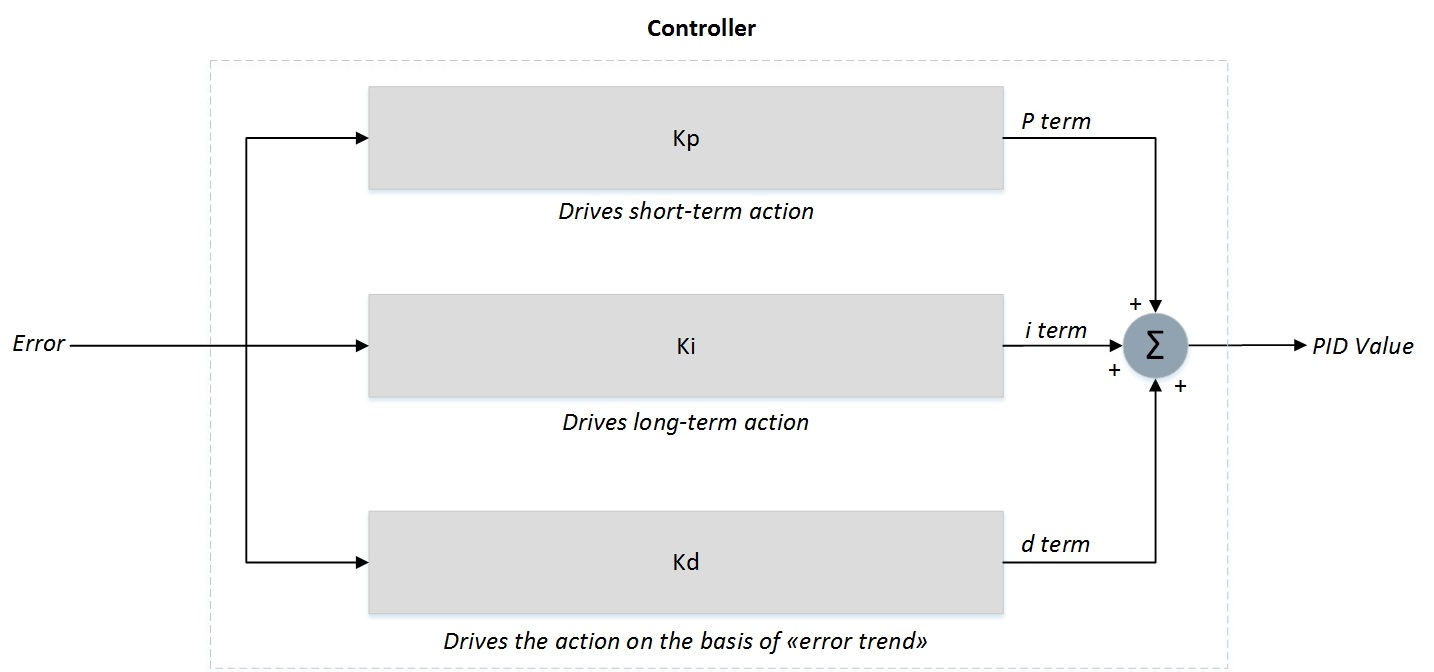
\includegraphics[scale = 0.7]{VAPIQ-PICTURES/pid.jpg}
            \caption{PID Controller}
            \label{fig:pid}
\end{figure}
The control system of both the fixed pitch quadrotor and the variable pitch quadrotor are based on PID controllers. Fig. \ref{fig:pid} shows a simple setup for a PID controller. A PID controller consists of a P-term for Proportional, a I-term for Integral and a D-term for Derivative. A PID controller continuously calculates an error value. This value is based upon the difference in desired position and actual position. Corrections are based on the sensor data.

\section{FPQ Control System}
Fig. \ref{fig:dir} shows the controller for the first FPQ concept. It is based on a PID controller, only using the P-term. It stabilizes the quadrotor by using accelerometer and gyro data. The gyro outputs data in $deg/s$ and the accelerometer in $m/s^2$. The input is a desired angle in pitch, roll and/or yaw direction.
\begin{figure}[H]
          \centering
            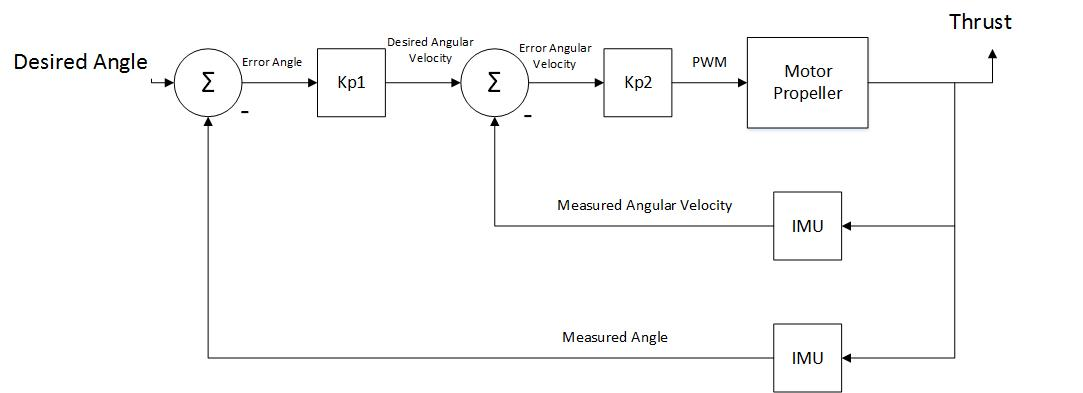
\includegraphics[scale = 0.5]{VAPIQ-PICTURES/CSBD.jpg}
                \caption{Proportional-Controller}
            \label{fig:dir}
\end{figure} 

A three-axis accelerometer can be used to calculate tilt angle by using trigonometry. \bigskip
By taking the desired angle of the quadrotor and subtracting the measured angle, the result is an error in angle.

\begin{equation}
   Angle Error = Desired Angle - Measured Angle
\end{equation}

The angle error is multiplied with a constant which results in desired angular velocity. 

\begin{equation}
   Desired Angular Velocity = Angle Error * Kp
\end{equation}

The gyroscope measures the actual angular velocity. Subtracting the measured velocity from the desired angular velocity gives the angular velocity error. 

\begin{equation}
   Angular Velocity Error = Desired Angular Velocity - Measured Velocity
\end{equation}

This error is multiplied with a constant which results in a PWM signal, sent to the motor.
\begin{figure}[H]
          \centering
            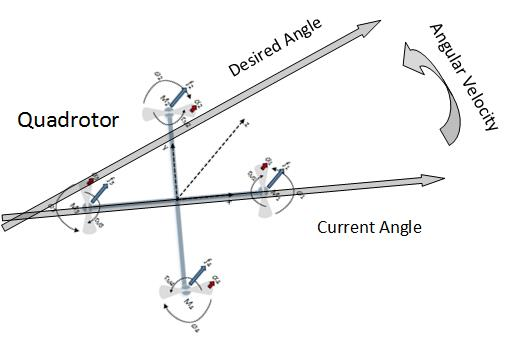
\includegraphics[scale = 0.67]{VAPIQ-PICTURES/OnBCS.jpg}
                \caption{Stability Control}
                \label{fig:Stab}
\end{figure} 

Fig. \ref{fig:Stab} shows the relationship between actual angle, desired angle and the angular velocity. 

\section{VPQ Flight Modes}
Flying the VPQ, two flight modes are available. The modes are acro-mode and auto-leveling mode. Acro-mode, means that the radio controller stick inputs are translated into commands for angular velocity. Auto-level mode also gives velocity rates, but when the sticks are released the quadcopter will return to level.

\subsection{Acro-Mode}

The variable pitch quadrotor control system uses a PID controller to achieve stabilization. 

Acro mode is the most agile flight mode, but requires some flight experience in order to properly control the quadcopter.\bigskip

%The control system is based on acro-mode control
%If the stick is released, then the quadrotor will maintain its current altitude and not lose its position. 
% The radio controller gives commands to the control system.

Fig. \ref{fig:micro} shows an overview of the control system in acro-mode. 

% SKAL VI SKRIVE OM HVORDAN MTOROR OG SERVO 
%MAPPINGA FOREGÅR OG HVA ER VINKEL PÅ PROPELL BLAD?


\begin{figure}[H]
          \centering
            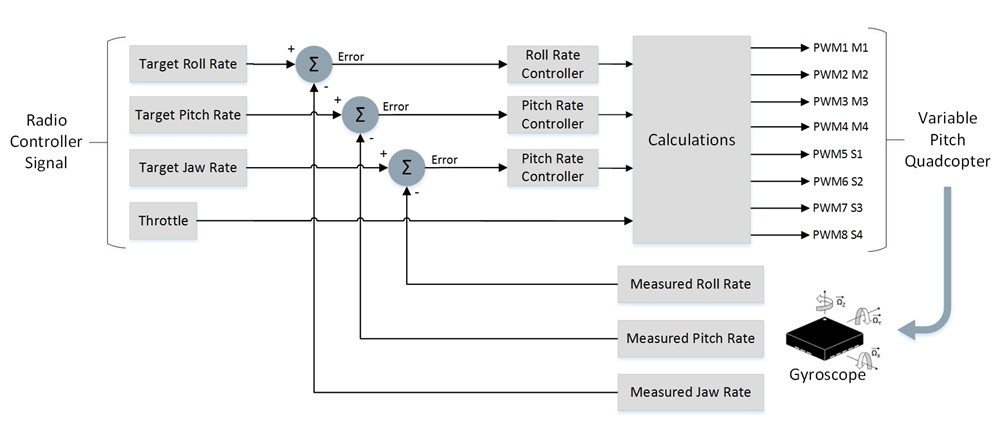
\includegraphics[scale = 0.55]{VAPIQ-PICTURES/controldrawing}
            \caption{Control system}
            \label{fig:micro}
\end{figure} 


Fig. \ref{fig:simple} shows a simplified version of the inputs and outputs to the microcontroller, in this case an Arduino Nano. The inputs to the control system are target rates, throttle, and the measured rates from the gyroscope. The difference between the inputs of the pilot and the gyro data results in an error, which the PID algorithm will try to compensate for. PWM signals are distributed to the corresponding motors for compensation. The signals are sent to both the motors and servos. The servos can change the propeller pitch angle between a set zero-pitch and 18 degrees. The PWM signals to the motors are limited between 1300 and 1500 microseconds. The start value corresponds to a rotational speed of 8000 RPM. Increasing the throttle results in a propeller pitch change and a compensation in motor velocity, which in turn yields thrust. 

\begin{figure}[H]
          \centering
            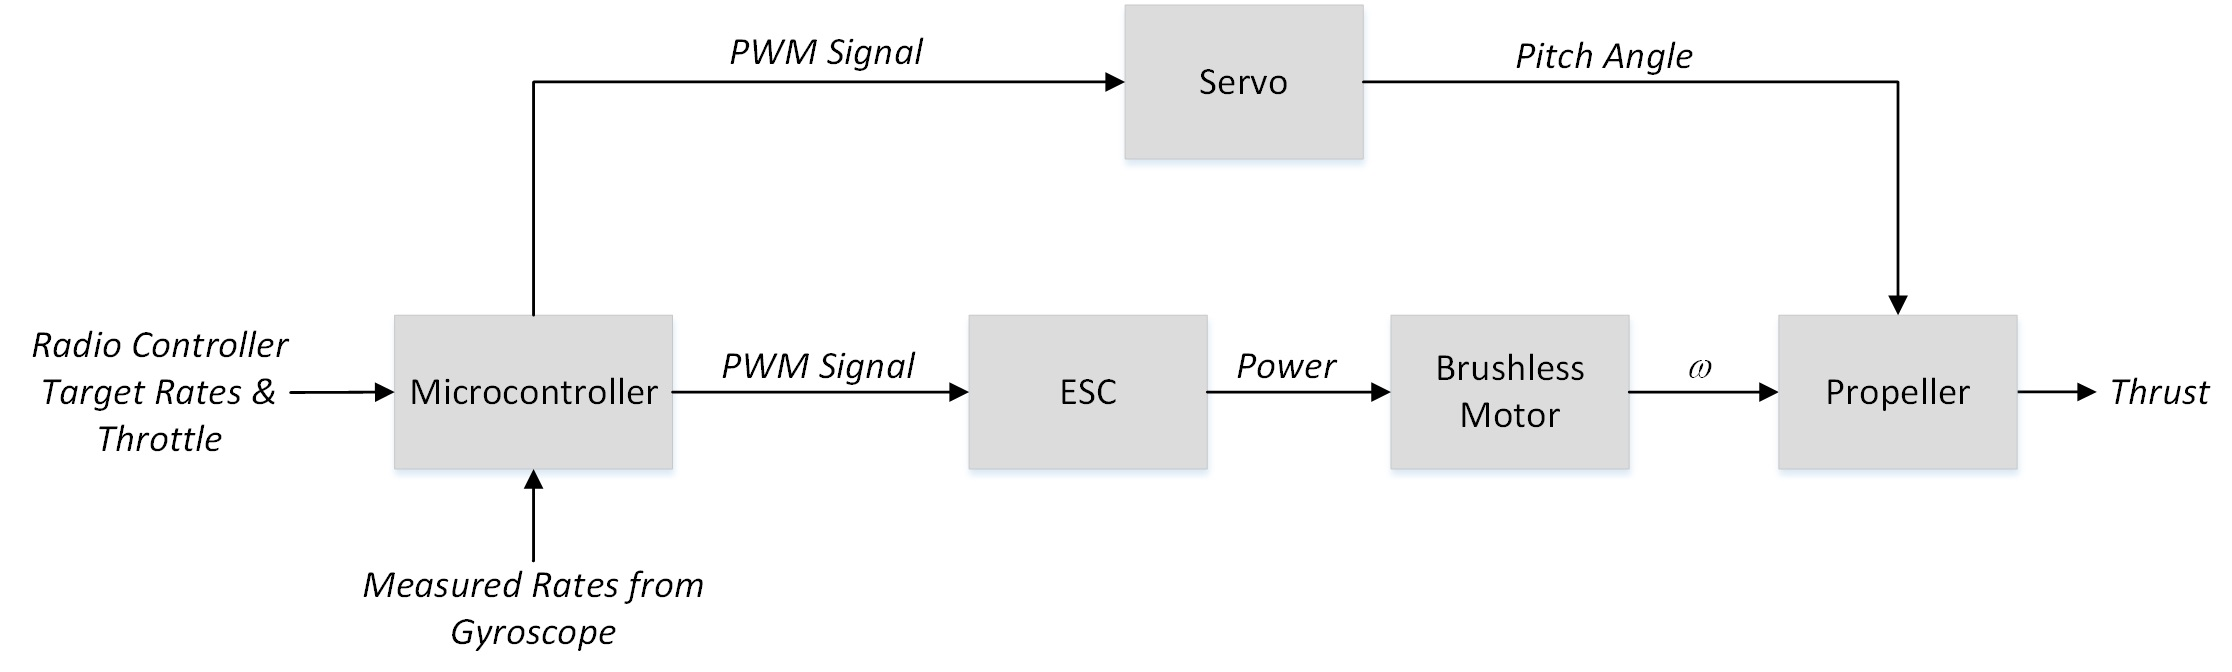
\includegraphics[scale = 0.45]{VAPIQ-PICTURES/simpleloop.jpg}
            \caption{Simplified thrust logic}
            \label{fig:simple}
\end{figure} 


\subsection{Auto-Level Mode}
Auto-leveling mode utilizes both the gyroscope and the accelerometer to calculate error in position. In this mode, the accelerometer is also used to counteract the drift that occurs in the gyro over time.
\\
In auto-level mode, when the RC sticks are released, the quadcopter stabilizes to level position. It uses the accelerometer to identify the direction of the gravitational vector, and based upon the direction it can identify and return to level position. 
\\
The direction of gravity is found with the following equation:

\begin{equation}
    acc\_total\_vector = sqrt((acc\_x*acc\_x)+(acc\_y*acc\_y)+(acc\_z*acc\_z)); 
\end{equation}

The angle in pitch can then be given as a sin function of the force in pitch or yaw divided by the total force. 

\begin{equation}
    angle\_pitch\_acc = asin((float)acc\_y/acc\_total\_vector)* 57.296;
\end{equation}

\begin{equation}
    angle\_roll\_acc = asin((float)acc\_x/acc\_total\_vector)* -57.296;
\end{equation}

The Arduino asin function outputs in radians, this is why it is multiplied with the conversion factor 57.296. Radians are converted to degrees by multiplying with 1/($\frac{\pi}{180}$) = 57.296. \bigskip 

%To remove the offset on the accelerometer it has to be calibrated in the start-up phase. When the data is clean and filtered it can be used to calculate the gyro angle drift.
%For the gyro, the traveled angle needs to be calculated. The gyro from MPU6050 is 65.5 when it is moving one degree per second.
% and the control loop is running at 250 Hz. 
%This means that a conversion is needed to get the rotational angles. 
The gyro in MPU6050 outputs 65.5 when it is moving one degree/s. The traveled angles can be found from the conversion factor 1/(250*65.5) multiplied with the gyro values. In the conversion, 250 is the loop frequency in Hz. These values are added to the angle\_roll and angle\_pitch variables. Added over time this will give the traveled angles.
%Adding the gyro data over time is integrating, and the integral of degrees/s will be the degrees traveled.

\begin{equation}
    angle\_pitch += gyro\_pitch * 0.0000611;
\end{equation}

\begin{equation}
    angle\_roll += gyro\_roll * 0.0000611;     
\end{equation}                           

If the quadcopter is at an incline and yawing, the the sensor cannot detect pitch and roll, the values will almost not change. This is because there is little to none angular motion in the pitch and roll directions. In order to compensate for this,  the pitch and roll angle must be transferred based upon the change in yaw. The transformation is done with a simple sin function. The arduino sin function takes radians as input, so we need to take the previously calculated number (0.0000611) and convert it to radians by multiplying with $\frac{\pi}{180}$.

\begin{equation}
    angle\_pitch -= angle\_roll * sin(gyro\_yaw * 0.000001066);
\end{equation}      

\begin{equation}
    angle\_roll += angle\_pitch * sin(gyro\_yaw * 0.000001066);     
\end{equation}      

To correct for gyro drift, a small part of the accelerometer data is needed to compensate, this is done by using a complementary filter. .As little as 0.04\% of the data is enough for corrections. \cite{gyroDriftTemp} \\
This number was found by analyzing the gyro data and experimenting with the parameters of the complementary filter.

\begin{equation}
    angle\_pitch = angle\_pitch * 0.9996 + angle\_pitch\_acc * 0.0004;
\end{equation}

\begin{equation}
    angle\_roll = angle\_roll * 0.9996 + angle\_roll\_acc * 0.0004; 
\end{equation}                     

Under flight, the quadcopter has an angle limit. This limit is adjusted by multiplying the pitch and roll angles with a constant. The larger the constant the lower the angle allowed. This constant is set to 18 in the variable pitch flight controller, which gives a max tilt angle of approximately 27 degrees.

\begin{equation}
    pitch\_level\_adjust = angle\_pitch * 18;
\end{equation}

\begin{equation}
    roll\_level\_adjust = angle\_roll * 18;   
\end{equation}       

This pitch and roll adjustment is taken into the PID calculations and a pid\_error value gets calculated for each rotational angle. An example of how the PID calculation works is given below:\bigskip

$
pid\_output\_roll = pid\_p\_gain\_roll * pid\_error\_temp + pid\_i\_mem\_roll + pid\_d\_gain\_roll * (pid\_error\_temp - pid\_last\_roll\_d\_error);
$


%%%%%%%%%%%%%%%%    AUTONOMOUS BLABLA SE PÅ  %%%%%%%%%%%%%%%%%%%%%%%%%%%%%%%%%%%%%%%%%%%%%%%%%%%%%%%%%%%%%%%%%%%%%%%%%%%%%%%%

\section{Autonomous Control System}
The off-board control system computes the angles necessary to reach the desired position. This data is sent to the quadrotor. The autonomous system begins with storing the start position and the current time.
%% ANGLES OR/AND ROTATIONAL SPEED?
\bigskip
The external computer acquires the new position and rotation of the quadrotor with a refresh rate of 50 Hz. If no data is received a counter is increased, and the last position and rotation measured becomes the current. If this happens five times the quadrotor will stabilize and shutdown. If data is received the counter resets. \bigskip

When the off-board gets information from Qualisys, it calculates the current velocity. The last position and time is updated as the current time and position. \bigskip % Skriv litt om

\begin{figure}[H]
          \centering
            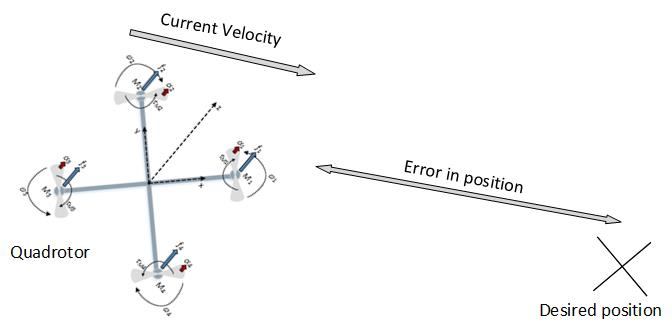
\includegraphics[scale = 0.67]{VAPIQ-PICTURES/OBCS.jpg}
                \caption{Trajectory Control}
                \label{TrajectoryControl}
            \label{fig:trajectory}
\end{figure} 

The next steps in this algorithm is very similar to how the fixed pitch quadrotor is stabilized. The first step is to calculate the error in position. This is done by taking the desired position and subtracting the current position.
\begin{equation}
   Error Position = Desired Position - Measured Position
\end{equation}

Multiplying the desired position with a constant yields the value for the desired velocity. 
\begin{equation}
   Desired Velocity = Error Position * Kp
\end{equation}

The desired velocity will then change regarding to the distance. The further away from the desired position, the bigger roll and pitch angles are desired. The error between the desired speed is found by subtracting desired velocity from the measured velocity.
\begin{equation}
    Error Velocity = Desired Velocity - Measured Velocity
\end{equation}

This error in speed can be directly applied to the roll and pitch angles when multiplied with another constant. 
\begin{equation}
   dAngle =  Error Velocity * Kp2
\end{equation}

The thrust also gets computed in this algorithm. To get the thrust vectors in the X and Y directions, the thrust given is divided by $\cos$ to the respective angles. The combined thrust vector is found by adding components for X,Y and Z. The Z component can be found by taking the error in Z-position times a constant.  
\begin{equation}
        ThrustX = \frac{thrust}{cos(angularX)}
\end{equation}

\begin{equation}
        ThrustY = \frac{thrust}{cos(angularY)}
\end{equation}

\begin{equation}
        Thrust = \frac{thrustX + thrustY}{2}  + errorZ*kpZ
\end{equation}

The values computed needs to be limited in order to not exceed angles that cannot be flown in.
All the data computed in the algorithm then gets sent to the quadrotor and the code rinse and repeats.

% \section{PID Tuning}
% To achieve stable flight, the control system must be tuned properly. This is done by identifying the correct PID-values through a combination of methods, trial and error. In the flight controller, there are three PID-loops for each of the rotational directions; roll, pitch and yaw. \bigskip

% % To get a stable quadcopter, the control system must be properly tuned. To do this, the right PID-values must be identified.
% % The PID values have been obtained by means of testing, trial and error \cite{PID-tune}.
% % \\
% % The PID controller has three parameters that must be tuned P, I and D. In the flight controller there are three different PID- loops. Each of the rotational directions pitch, roll and yaw.

% %The PID can be tuned by changing the parameters of each PID controller. The YMFC code have three such PID controllers, one for pitch, one for roll and one for yaw.
% % \\
% % \\
% % When tuning these parameters start with pitch and roll at zero.
% % \\
% % \\
% The approach used to tune the PID-controller is given below:
% \begin{itemize}
%     \item \textbf{Yaw}
%         \begin{itemize}
%             \item  Eliminate uncontrolled yaw by increasing the proportional value by one, until yawing stops.
%             \item  Increase the integral value by 0.01 to prevent yaw impact from small physical differences. %to what value
%             \item  For yaw, there is no need to change the derivative value because of the drag generated from the propellers.
%             %why?
%         \end{itemize}
%     \item \textbf{Roll and Picth} are given the same value unless the quadrotor has a CG outside of physical center.
%         \begin{itemize}
%             \item The derivative value is increased by one until the quadrotor shows high frequency oscillations, then lowered down until the quadcopter runs smooth again. The value is then reduced by 25\%. 
%             \item The proportional value is increased by 0.2 until the quadrotor starts to overcompensate, then divide the value by 2.
%             \item The integral value is changed by 0.01 until the quadrotor starts to oscillate, then divide by 2.
%             \item Increasing the proportional value until fast oscillation occur, and subtract a few points until the quadcopter is fully stable. 
%         \end{itemize}
% \end{itemize}

% By following these steps, the quadrotor should be stable and able to fly. To get the variable pitch properly tuned, the method above was applied and additional advise was taken from a professional RC pilot. The final PID settings for the variable pitch quadrotor for pitch and roll are (11.5, 0.03, 10) and the values for yaw are (18, 0.04, 0) \cite{PID-tune}.

% The first goal is to eliminate the yaw effect of the quadrotor. This can be done by increasing thrust until it almost lifts and see which way it yaws. The proportional value is then incremented by one and one until the quadrotor is not yawing.
% \\
% \\
% The next parameter to change is the integral value for yaw. The value is incremented by 0.01. This is done to prevent yaw impact from small physical differences. The derivative value in for yaw is not needed since the propellers generate drag. The yaw PID parameters found for the variable pitch quadrotor is {18, 0.04, 0}.
% \\
% \\
% The pitch and roll are then changed and will have the same value unless the quadrotor has a center of gravity outside of the physical centre of the quadrotor.
% \\
% \\
% The YMFC joop method differs a little in contradiction to the famous and well known Ziegler–Nichols PID tuning method. Ziegler Nichols method, the derivative value is the first to be changed after yaw. \cite{Ziegler-Nichols1} \cite{Ziegler-Nichols2}
% \\
% \\
% The derivative value for pitch and roll is increased by one and one until the quadrotor becomes restless i.e high frequncy movements. The value is then divided by 25 percent, and this parameter is obtained.
% \\
% \\
% The proportional value is increased by 0.2 for each test. The value is divided by 50 percent when the quadrotor starts to over compensate.
% \\
% \\
% At last the Integral value is changed by 0.01. This is done until the quadrotor starts to oscillate, when this happens the value is divided by 50 percent.
% \\
% \\
% Increase the proportional value again for the pitch and roll up to the point of fast oscillations. Then take it back a few points.
% \\
% \\
% The quadrotor should now be possible to fly sub-optimal. For the variable pitch quadrotor the PID values for pitch and roll is {11.5, 0.03, 10}. The PID values can further be tuned with minor changes to perfect the PID controller.\cite{PID-tune}
